\documentclass[a4paper]{article}

\usepackage[T1]{fontenc}
\usepackage[italian]{babel}
\usepackage[latin1]{inputenc}
\usepackage{graphicx}
\usepackage{float}
\usepackage[margin=2 cm]{geometry}
\usepackage{multirow}
\usepackage{multicol}
\usepackage{textcomp}
\usepackage{caption}
\author{Alberto Bordin, Giulio Cappelli}
\title{Duplicatore di frequenza}
\date{14-15 Dicembre 2017}
\newcommand{\minitab}[2][l]{\begin{tabular}#1 #2\end{tabular}}


\begin{document}
	\maketitle
	
	\begin{abstract}
		 
	\end{abstract}

\section{To do}
	
\section{Teoria}

\section{Apparato sperimentale}

\section{Taratura}

\begin{multicols}{2}
	Per prima cosa abbiamo tarato l'attenuatore regolabile. Abbiamo misurato la potenza ogni 5 gradi centesimali. I dati raccolti sono riportati in appendice (Tabella \ref{tab:taratura}) e graficati in Figura \ref{fig:taratura}.
	
\subsubsection*{Discussione degli errori}
In Figura \ref{fig:taratura} abbiamo distinto errore di calibrazione ed errore statistico; nelle misure delle prossime sezioni verr� usato il primo o il secondo a seconda delle esigenze. L'errore di calibrazione � dato dall'accuratezza riportata nel datasheet del sensore del \textit{power meter}. L'errore statistico � stato stimato guardando le fluttuazioni delle differenze tra misure di potenza consecutive (vedi Figura \ref{fig:differenze_taratura} e relativa didascalia).

\end{multicols}

\begin{figure}[H]
	\centering
	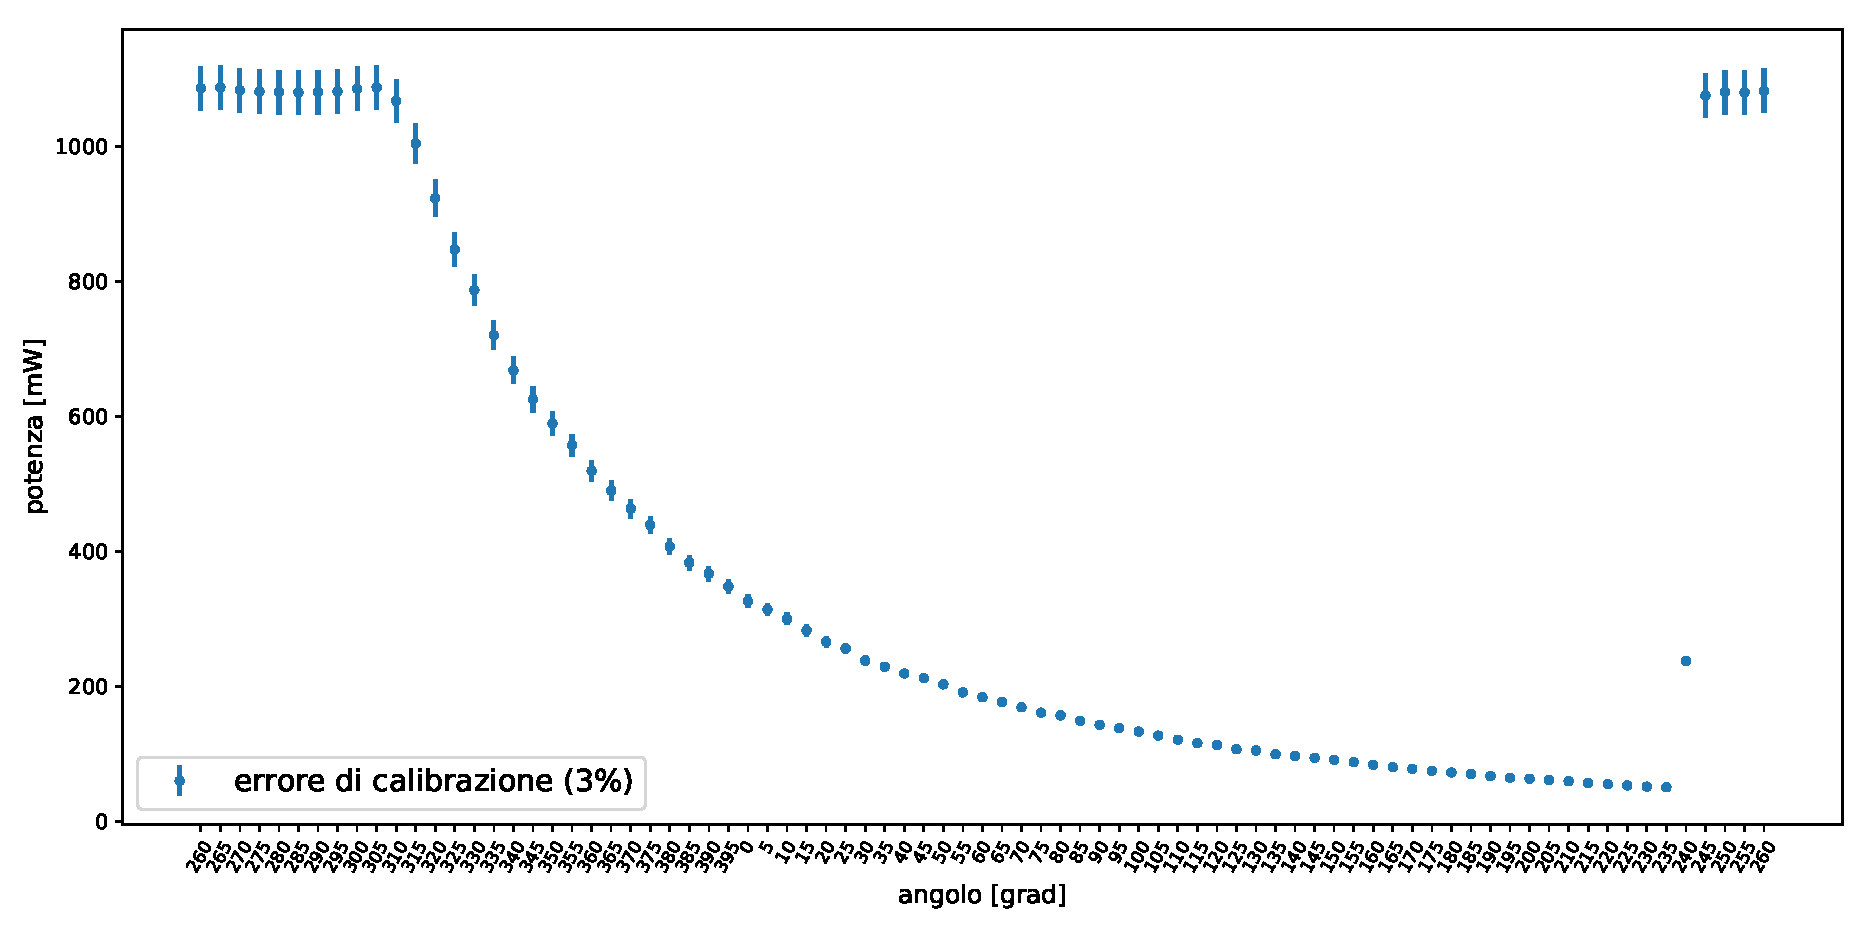
\includegraphics[width=1\textwidth]{taratura.pdf}
	\caption{Taratura dell'attenuatore regolabile.}
	\label{fig:taratura}
\end{figure}

\begin{figure}[H]
	\centering
	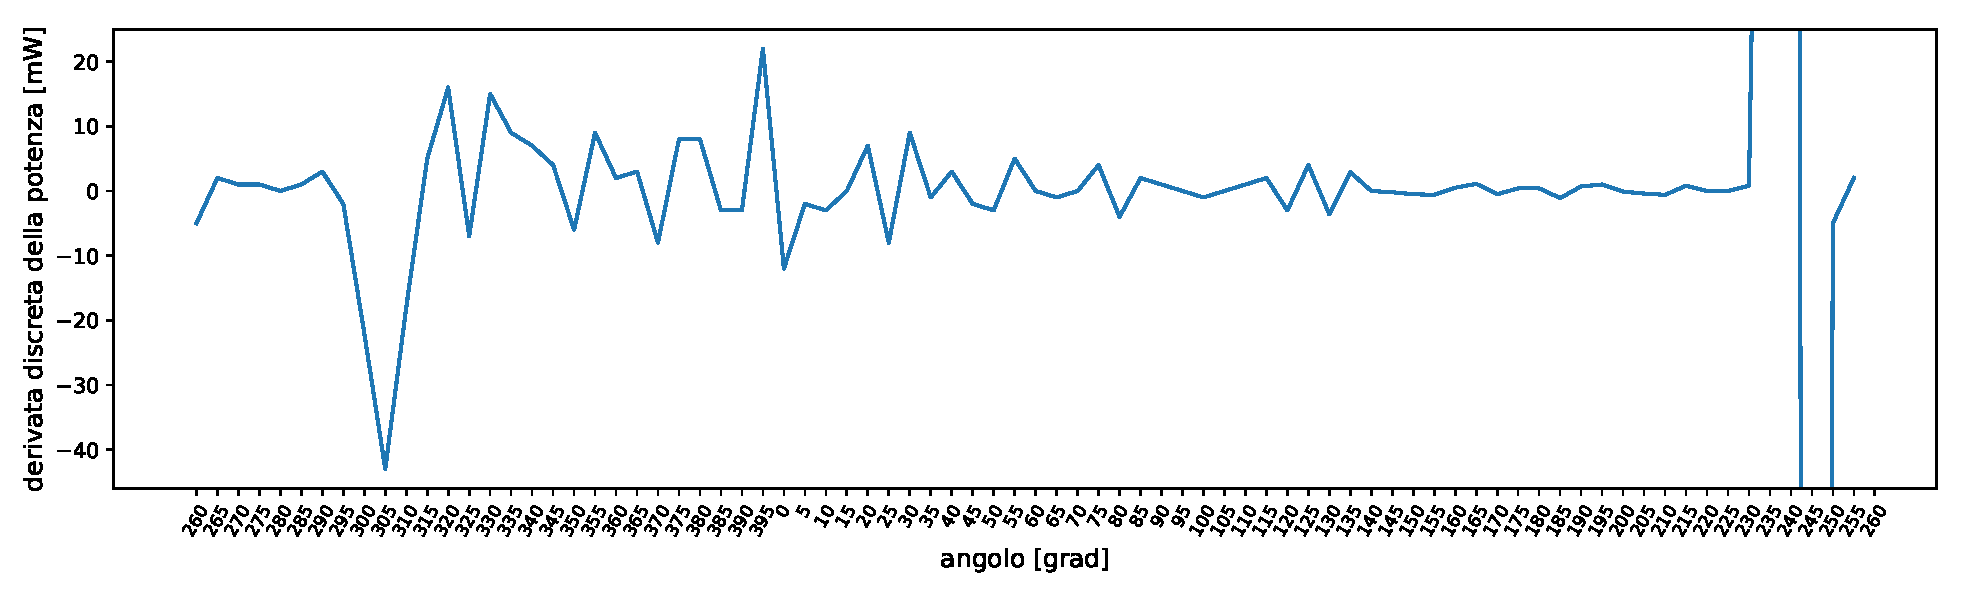
\includegraphics[width=1\textwidth]{fluttuazioni_differenze_taratura.pdf}
	\caption{Derivata discreta della curva della taratura dell'attenuatore. Le fluttuazioni sono circa dell'1\% della potenza. A 240 grad la curva di taratura presenta una discontinuit� nella derivata, pertanto i punti tra 230 e 250 grad non sono stati considerati per la stima dell'errore statistico.}
	\label{fig:differenze_taratura}
\end{figure}

\section{Segnale duplicato in funzione della potenza incidente}

\subsection{Presa dati}

1 tabella

\subsection{Analisi dati}

2 fit ax$^b$ e ax$^2$

\section{Angolo di phase-matching}

\subsection{Presa dati}

1 tabella

\subsection{Analisi dati}

1 fit a tutti a dati, 1 fit con un cut sulle code e 2 fit con gaussiana e parabola

\section{Polarizzazione}

\subsection{Presa dati}

\subsubsection{Polarizzazione in ingresso}

1 tabella

\subsubsection{Polarizzazione in uscita}

1 tabella

\subsection{Analisi dati}

\subsubsection{Polarizzazione in ingresso}

1 fit

\subsubsection{Polarizzazione in uscita}

1 fit

\newpage
\section*{Appendice}

\begin{table}[H]
	\centering
	\begin{tabular}{|cc|cc|cc|cc|cc|}
		\hline
		$\Theta$ [grad] & P [mW] & $\Theta$ [grad] & P [mW] & $\Theta$ [grad] & P [mW] & $\Theta$ [grad] & P [mW] & $\Theta$ [grad] & P [mW] \\
		\hline
		260 & 1086 & 345 & 625 & 30 & 238 & 115 & 116 & 200 & 63.1 \\
		265 & 1087 & 350 & 589 & 35 & 229 & 120 & 113 & 205 & 61.5 \\
		270 & 1083 & 355 & 557 & 40 & 219 & 125 & 107 & 210 & 59.5 \\
		275 & 1081 & 360 & 519 & 45 & 212 & 130 & 105 & 215 & 56.9 \\
		280 & 1080 & 365 & 490 & 50 & 203 & 135 & 99.4 & 220 & 55.1 \\
		285 & 1080 & 370 & 463 & 55 & 191 & 140 & 96.7 & 225 & 53.3 \\
		290 & 1080 & 375 & 439 & 60 & 184 & 145 & 94.0 & 230 & 51.5 \\
		295 & 1081 & 380 & 407 & 65 & 177 & 150 & 91.1 & 235 & 50.5 \\
		300 & 1085 & 385 & 383 & 70 & 169 & 155 & 87.7 & 240 & 237.4 \\
		305 & 1087 & 390 & 367 & 75 & 161 & 160 & 83.7 & 245 & 1075 \\
		310 & 1067 & 395 & 348 & 80 & 157 & 165 & 80.2 & 250 & 1080 \\
		315 & 1004 & 0 & 326 & 85 & 149 & 170 & 77.8 & 255 & 1080 \\
		320 & 923 & 5 & 314 & 90 & 143 & 175 & 74.9 & 260 & 1082 \\
		325 & 847 & 10 & 300 & 95 & 138 & 180 & 72.4 &  &  \\
		330 & 787 & 15 & 283 & 100 & 133 & 185 & 70.3 &  &  \\
		335 & 720 & 20 & 266 & 105 & 127 & 190 & 67.1 &  &  \\
		340 & 668 & 25 & 256 & 110 & 121 & 195 & 64.6 &  &  \\
		\hline
	\end{tabular}
	\caption{Taratura dell'attenuatore regolabile. Gli errori di calibrazione sulle potenze sono del 3\%, quelli statistici dell'1\%. L'errore sull'angolo � inferiore a 0.5 gradi centesimali, quindi � trascurabile.}
	\label{tab:taratura}
\end{table}



 
\end{document}